\documentclass{article}
\usepackage[utf8]{inputenc}
\usepackage{graphicx}
\graphicspath{ {imagenes/} }
\setlength{\parskip}{5mm}

\title{Práctica entregable de los bloques 3 y 4: 
\newline LATEX, git, python, Numpy, Matplotlib, gdb y profiling}
\author{ Victor Espín Belmonte y Jaime Ortiz Aragón }
\date{April 2020}

\begin{document}

\maketitle

\section{Planteamiento del problema}
La resolución de los Bloques III y IV de la asignatura constan de desarrollar un programa propuesto en Phyton y C, ayudándonos de las estructuras que se nos han proporcionado en las presentaciones de teoría \textit{LatexTeoria.pdf, GitTeoria.pdf, PythonTeoria.pdf y teii-bloque4.pdf} así como en las estructuras del código en \textit{bloque4-codigo.tgz}. La implementación del código la hemos ido recopilando en la aplicación \textbf{github.com} con el fin de haber podido mostrar nuestro progreso, el cual hemos ido realizando a la par por videollamadas de \textbf{Skype}.

En concreto, el problema a resolver en esta tarea consistía en dada una lista de tamaño variable de entrada, controlar los elementos repetidos que contiene, en nuestro caso \textit{int}, para proporcionar como salida una lista sin repetidos.

Estos valores pueden variar en el intervalo \textbf{[0-99999]} y la longitud de la lista puede ser de hasta \textbf{200000} valores, siendo el valor máximo el que se establece como referencia en el enunciado de la tarea.


\section{Resolución del problema}
\subsection{Generación aleatoria de números}
El primer paso que realizamos para la confección del problema consistió en comprobar los argumentos que debía recibir el programa : los argumentos de entrada para generar el fichero con los números de la lista completa son el nombre del fichero y el número de enteros que contiene.

Para generar en \textit{Phyton} el fichero con la lista de números aleatorios hicimos uso de la librería \textit{Numpy}, que nos permite mediante la función \textit{np.random.randint(valormax)} generar un número en el intervalo \textbf{[0-valormax]}. Para que esto generara la lista, simplemente debíamos realizar dicha operación para cada elemento, con su escritura en el fichero pasado como parámetro.

Este código se encuentra en el fichero \textit{Fichero.py} en la carpeta de \textit{Phyton}.

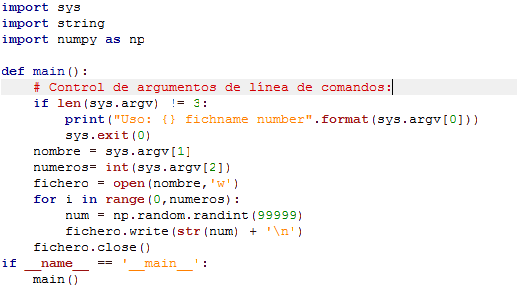
\includegraphics[width=11.5cm]{fichero.PNG}

Aquí podemos ver la captura del codigo. Como se extraen los argumentos y como se genera el fichero con el bucle for que genera números aleatorios.

\subsection{Programa principal en \textit{Phyton}}
El programa principal, que se encuentra en el fichero \textit{Practica3.py}, recibe como parámetros el nombre del fichero que se generó en el apartado \textbf{2.1}, el fichero en el que va a escribir la lista de números sin repeticiones y el fichero pdf en el que se va a guardar la gráfica que se nos pide representar.

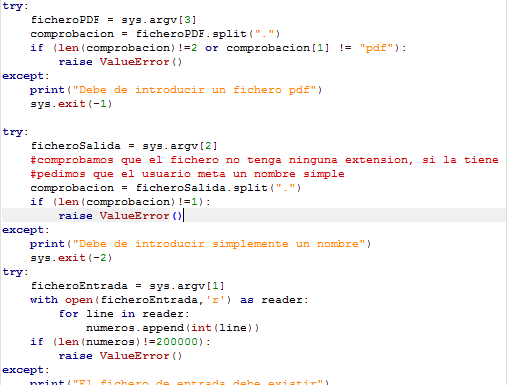
\includegraphics[width=11.5cm]{Tratamiento_Errores.PNG}

En esta imagen podemos ver como se trata que los parámetros de entrada sean o no correctos. Primero vemos como comprobamos utilizando split que la extensión del fichero para el pdf sea .pdf, si esto no es así acabaremos con un error. Después comprobamos que el fichero de salida, en el que se escriben los números sin repeticiones, no tenga ninguna extensión rara también con split. Si el fichero tiene una extensión abortamos. Finalmente para comprobar que el fichero de entrada tiene doscientos mil números simplemente metemos todas las líneas en una lista y comprobamos que su longitud sea de doscientos mil elementos.

Se nos pide que resolvamos el problema de dos formas distintas y tras estudiar órdenes de complejidad, nos decantamos por utilizar conjuntos y diccionarios. Ambos presentan un \textbf{O(n)} en sus operaciones para eliminar los repetidos. Por definición, un conjunto es una colección de valores que no presenta repetidos, por lo que si pasamos una lista a un conjunto, en este podremos encontrar todos los valores de la lista eliminando los repetidos. Esto lo realizamos en la línea \textit{list(set(aux))}, que transforma la lista \textit{aux} en un conjunto y posteriormente en una lista de nuevo, con los valores del conjunto. 

Por otra parte, en Python, un diccionario es una colección no-ordenada de valores que son accedidos a través de una clave. Estos tipos pueden ser listas, cadenas, tuplas, otros diccionarios, objetos, etc. Como es de esperar, una tupla no puede estar repetida, ya que cada clave hace referencia a una tupla del diccionario. Para conseguir pasar una lista con elementos repetidos a un diccionario solo debemos usar \textit{dict.fromkeys(aux).keys()}. Esto lo haremos en un bucle while en el que se irán procesando cada vez mas elementos de la lista, concretamente dos mil más en cada iteración.

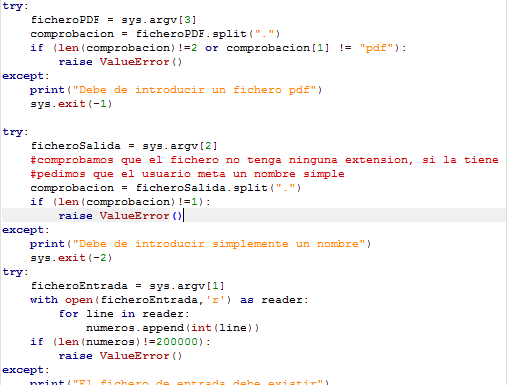
\includegraphics[width=11.5cm]{Tratamiento_Errores.PNG}

En la imagen vemos como transformamos la lista en un set y en un diccionario. De esta forma eliminamos elementos repetidos. También podemos ver como calculamos los tiempos en los que esta transformación se lleva a cabo.

Otra solución que podríamos haber adoptado son el ordenar la lista e ir buscando si el elemento \textit{n} es igual al \textit{n+1} para ir eliminando. Otra más podría haber sido tener un array de \textbf{0-valormax}, y cuando vayamos encontrando un valor, marcarlo como encontrado en el array.

Como cabe de esperar, el orden de magnitud es mucho mayor al adoptado en nuestras soluciones.

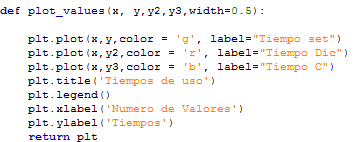
\includegraphics[width=11.5cm]{dibujarGrafica.PNG}

En esta función auxiliar podemos observar como utilizando matplotlib podemos dibujar una gráfica. En las tres primeras lineas dibujamos las líneas correspondientes a los tres métodos. Seguidamente colocamos el titulo y una leyenda. Para finalizar con la gráfica le damos nombre a los dos ejes.

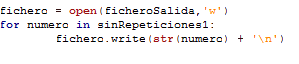
\includegraphics[width=11.5cm]{EscrituraFichero.PNG}

Antes de pasar a explicar como funciona el uso de la librería ctypes para utilización de código C en python, vemos como para terminar el programa se escribe la lista de números sin repeticiones en el fichero de salida.

Finalmente hay que indicar que antes de poder ejecutar el programa como tal habrá que ejecutar el programa Fichero.py con un nombre de fichero y 200000 como segundo argumento. También habrá que hacer make en la carpeta de C para que se cree la librería necesaria.

\subsection{Programa principal en C}
Para pasar el código de \textit{Phyton} a \textit{C} nos hemos basado en el fichero que se nos ofreció \textit{mult.py}.

Dado que se nos pide que la reserva de memoria se haga en \textit{Python}, debemos conseguir hacer desde aquí una llamada al código \textit{C}, que se encontrará en la carpeta C correspondiente.

En nuestro fichero \textit{Listas.py} utilizamos la biblioteca de \textit{Ctypes}.

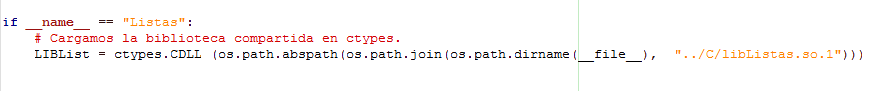
\includegraphics[width=11.5cm]{definicion.PNG}

Para cargar la biblioteca compilada por nuestro makefile usaremos la librería os de python y le pasaremos la ruta.

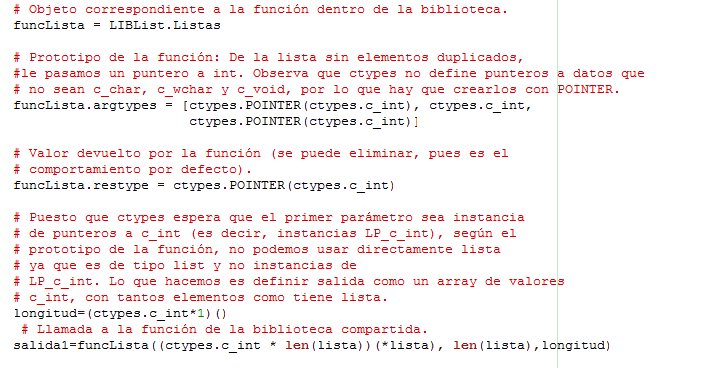
\includegraphics[width=11.5cm]{ctypes1.PNG}

En la primera línea podemos ver como se carga la función en c dentro de la biblioteca. Después definimos los parámetros de la función. Estos parámetros tienen que estar dentro de los tipos de ctypes. En este caso utilizaremos ctypes.Pointer(ctypes.cint) para el primer y el tercer argumento, lo que nos indica que serán punteros a enteros como veremos más adelante. Para el segundo parámetro simplemente indicaremos que será un ctypes.cint indicando que es un entero.

Siguiendo con la imagen podemos ver como definimos el tipo de retorno de la función como un puntero de enteros, que será la lista sin repeticiones. Para terminar con esta imagen vemos como definimos que el tercer parámetro sea un array de una sola posición, esto lo hacemos así por que necesitamos almacenar la longitud de la lista sin repeticiones para recorrerla posteriormente. También podemos ver como llamamos a la función con todos sus parámetros correspondientes.

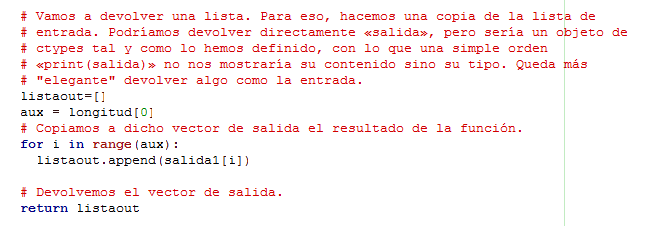
\includegraphics[width=11.5cm]{ctypes2.PNG}

Finalizando con Listas.py tenemos como devolver la lista sin repeticiones. Extraemos la longitud de la lista sin repeticiones del tercer parámetro de la función. Con este dato recorremos toda la lista de salida introduciendo los datos en una lista de python para devolverla posteriormente

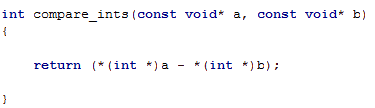
\includegraphics[width=11.5cm]{Comparacion.PNG}

Antes de pasar a la función principal en C tenemos esta función auxiliar que pasaremos a la función qsort como parámetro para ordenar la lista, ya que esto nos bajara el orden de la función bastante. Esta función lo único que hace básicamente es devolver la resta entre los dos números para saber cual es mayor de los dos.

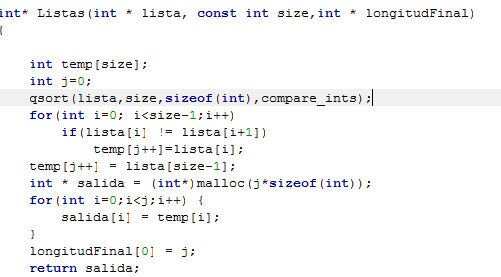
\includegraphics[width=11.5cm]{C.PNG}

Finalmente para el algoritmo en C primero ordenamos la lista, después simplemente iremos recorriendo toda la lista y comprobando si el siguiente elemento es distinto al que tenemos. Si lo es simplemente tendremos que colocarlo en la lista de salida. Para terminar creamos una lista del tamaño preciso para eliminar los posibles residuos que nos hayan quedado.

\subsection{Comparación de tiempos de operaciones}
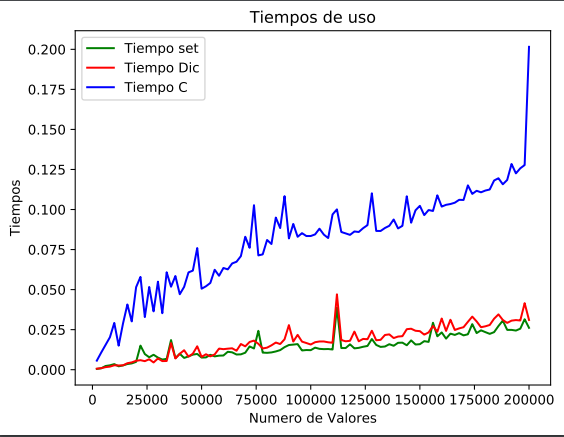
\includegraphics[width=11.5cm]{PDF.PNG}

Como era de esperar aun que el orden de nuestro programa en c es el orden de qsort, que debería estar en torno a nlogn, las soluciones de python son mucho mas eficientes. Esto es así por que estarán implementadas de una mejor manera usando hash o con algoritmos mucho mas eficientes. Para hacer un buen uso de la biblioteca ctypes es necesario plantear muy bien en que problema puede ser beneficioso, dado que si hay algún método o librería ya disponible en python es probable que no sea rentable usarla.

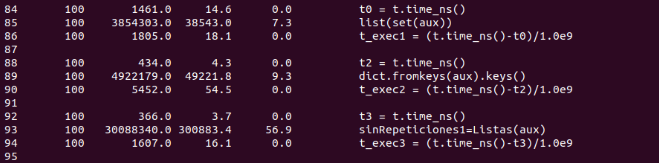
\includegraphics[width=11.5cm]{Line_profile.PNG}

En esta imagen podemos ver el uso de la herramienta line profile para el calculo del tiempo de ejecución de las funciones. En la primera columna podemos ver el numero de linea en el programa. En la segunda columna el número de veces que entra a esa linea. Finalmente en las dos siguientes columnas podemos ver el tiempo total que utiliza cada linea y el tiempo por entrada a esa linea respectivamente. Como podemos comprobar la llamada a la función en C es la que mas tiempo usa, un con algo mas de la mitad del tiempo de ejecución, mientras que el tiempo del set es algo menos que el de los diccionarios. Todo esto ya lo podíamos ver en el pdf que genera el programa automáticamente.

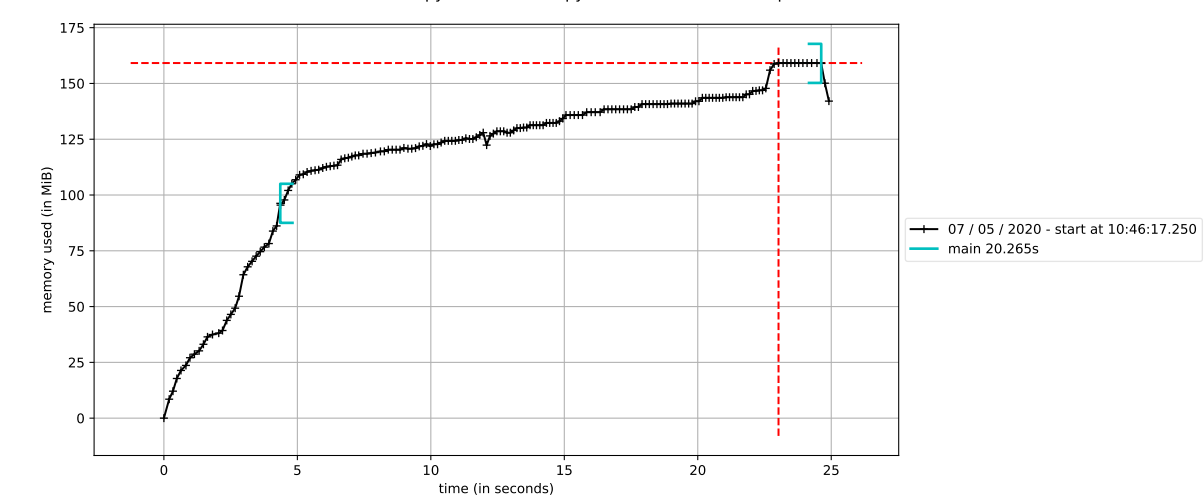
\includegraphics[width=11.5cm]{memory_profile.PNG}

Finalmente para terminar con el estudio del programa tenemos el estudio de la memoria. Como podemos ver el gran uso de memoria se debe al main. Esto es así por que en esta función es donde se crean tanto los nuevos sets y los nuevos diccionarios a parte de que es donde se reserva toda la memoria que se va a utilizar en C mediante el uso de ctypes. Es por esto que es de lo más normal del mundo que haya un crecimiento tan alto en esta parte del programa.

\end{document}
